\documentclass{article}
\usepackage[UTF8]{ctex}
\title{自适应宽度弧线与波浪线}
\author{Marlin}
\date{April 2018}

\usepackage{ifthen} 
\usepackage{amsmath,bm}
\usepackage{tikz}
\usepackage{scalerel}
\usepackage{stackengine}
\stackMath
%\stackText

\newcommand\reallywidefrown[1]{%
\stackon[0.5pt]{#1}{%
\stretchto{%
  \scaleto{%
    \scalerel*[\widthof{#1}]{\mkern-1.5mu\frown\mkern-2mu}%
    {\rule[-\textheight/2]{1ex}{\textheight}}%
  }{\textheight}%
}{0.8ex}}%
}
\newlength{\lmax}%
\newlength{\lfenzi}%
\newlength{\lfenmu}%
\newcommand\reallywidesim[2]{%
	\savestack{\fenzi}{\(#1\)}%
	\savestack{\fenmu}{\(#2\)}%
	\settowidth{\lfenzi}{\fenzi}%
	\settowidth{\lfenmu}{\fenmu}%
    \ifthenelse{\lengthtest{\lfenzi > \lfenmu}}
       {\setlength{\lmax}{\lfenzi}}
       {\setlength{\lmax}{\lfenmu}}
	\stackon[0.5pt]{\fenmu}{\stackunder[0.5pt]{\fenzi}{%
		\stretchto{%
			\scaleto{%
				\scalerel*[\lmax]{\mkern-1.5mu\sim\mkern-2mu}%
				{\rule[-\textheight/2]{1ex}{\textheight}}%
			}{\textheight}%
		}{1ex}}}%
}

\parskip 1ex
\begin{document}
\maketitle

$$\reallywidefrown{zbcdefghi}$$

$$\reallywidefrown{zbcdefg}$$

$$\reallywidefrown{zbcde}$$

$$\reallywidefrown{zbc}$$

$$\reallywidefrown{zb}$$

$$\reallywidefrown{\Shortstack{\sin z}} = 0$$

$$\reallywidesim{r_1}{r_2}$$

$$\reallywidesim{r_1\leftrightarrow r_2}{r_3\div 2 }$$

$$\reallywidesim{r_1\leftrightarrow r_2}{r_3\div 2, r_1\leftrightarrow r_2}$$

$$\reallywidesim{r_1\leftrightarrow r_2, r_1\leftrightarrow r_2}{r_3\div 2}$$

\[
\begin{array}{@{}c@{}}
\bm{r_1\leftrightarrow r_2}\\
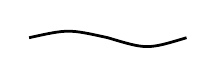
\begin{tikzpicture}
\draw[line width=1pt] (0,0) .. controls(.5,.11)..(1,0)
..controls(1.5,-.15) .. (2,0);
\end{tikzpicture}\\[-.5ex]
\bm{r_3\div 2}
\end{array}
\]

\end{document}
